\documentclass[twocolumn]{article}

%\usepackage[iso]{umlaute}
%\usepackage{german}
\usepackage{graphicx}
\setlength{\parindent}{0cm}
\setlength{\parskip}{1ex}
\setlength{\columnsep}{25pt}

\textwidth=17cm
\textheight=23cm
\setlength{\unitlength}{0.5cm}
\setlength{\parindent}{0.0cm}
\setlength{\parskip}{1ex}
\raggedbottom
\sloppy
%\addtolength{\evensidemargin}{-5cm}
\addtolength{\oddsidemargin}{-1.5cm}
\addtolength{\topmargin}{-2cm}

\sloppy

% Your name
\author{Trung Nguyen\\ Technische Universit\"at M\"unchen}

\title{Seminar Cloud Computing \\
       {\bf From Concept to Production: Enablements TinyML in Industrial Setting}
}

% Date of your talk
\date{November 2024}

\usepackage{hyperref}

\begin{document}

\maketitle

\begin{abstract}
In recent years, Artificial Intelligence (AI) and Machine Learning (ML) have received tremendous amount of attention in both industry and research world. However, conventional Machine Learning demands high computing capability which limits its usage to only larger computing units. The pardigm shift to Tiny Machine Learning (TinyML) is revolutionizing industries by enabling the deployment of machine learning models on low-power, resource-constrained devices. Being one of the most rapid developing field of Machine Learning, TinyML promises to benifits multiple industries. However, building a production-ready tinyML system poses different unique challenges. In this paper, we explore the key obstacles faced when developing and deploying TinyML models in production environments, including model optimization, hardware limitations, software integration, and maintaining performance in real-world conditions. Additionally, we present real-world use cases of TinyML in industrial settings, showcasing its transformative impact. We also discuss practical approaches and strategies presented by recent researches \cite{ren_tinyol_2021} to overcome these challenges, providing insights into how TinyML systems can be successfully scaled and implemented in production.
\end{abstract}

% \section defines numbered parts of the paper with titles
% there also are \subsection and \subsubsection
\section{Introduction}
\label{introduction}


Traditional Machine Learning Models, especially Deep Learning Models typically require substantial amount of computing capability to operate effectively. These models are often trained on powerful Graphics Processing Units (GPUs) and produce large models ranging from tens or hundreds of gigabytes (GB) down to smaller models in the range of 10 to 100 megabytes (MB). However, the memory requirements during runtime for these models far exceed what microcontrollers (MCUs) can handle.
The pardigm shift to TinyML is driven by the prevailing number of Microcontroller Units (MCU) currently circulating in the industry. According to a recent report \cite{noauthor_microcontroller_nodate,grandviewresearch_research_2023}, as of 2021, around 31 billion MCUs were shipped worldwide annually. The MCU market size is projected to increase in upcoming years \cite{noauthor_microcontroller_nodate}. This creates a big incentive for researchers and industry players to put effort into developing the technology further.
TinyML aims to enable data processing or inferencing directly on embedded systems, particularly on Internet Of Things (IOT), instead of streaming to the cloud. TinyML models can operate on energy- and memory-constrained devices by minimizing communication with external servers, using optimized architecture designs, and employing compression techniques such as quantization and pruning. The advancement of tinyML has positively influenced multiple industries and sectors such as: industrial IOT \cite{ray_review_2022}, healthcare \cite{bhamare_chapter_2024}, agriculture \cite{tsoukas_tinyml-based_2022}, IOT in smart-city \cite{hussein_original_2024,ray_review_2022}. \\[0.25cm]

Although various organizations have been actively investing resources into machine learning and data science projects, only around 13\% of these projects successfully progress to production.\footnotemark \footnotetext{\url{https://venturebeat.com/ai/why-do-87-of-data-science-projects-never-make-it-into-production/}} 
This low success rate highlights the complex challenges and gaps in translating ML concepts into fully functional, production-grade systems, especially in the realm of TinyML. In this paper, we aim to address these challenges and outline what is necessary to transition a TinyML project from concept to production, ultimately creating value for industrial applications. In Chapter~\ref{tinyml_overview}, we provide an in-depth overview of the fundamental concepts, techniques, and development pipeline of TinyML. Following this, in Chapter~\ref{prod_tinyml}, we draw on recent research to investigate the specific challenges encountered in developing and deploying TinyML models in production environments, as well as practical strategies to overcome these obstacles. Next, in Chapter~\ref{use_cases}, we explore real-world applications of TinyML in industrial settings, illustrating its transformative potential. Finally, in Chapter~\ref{future_of_tinyml}, we consider the future trajectory of TinyML, discussing upcoming advancements and their implications for broader industrial adoption.
\begin{figure}
	\centerline{
	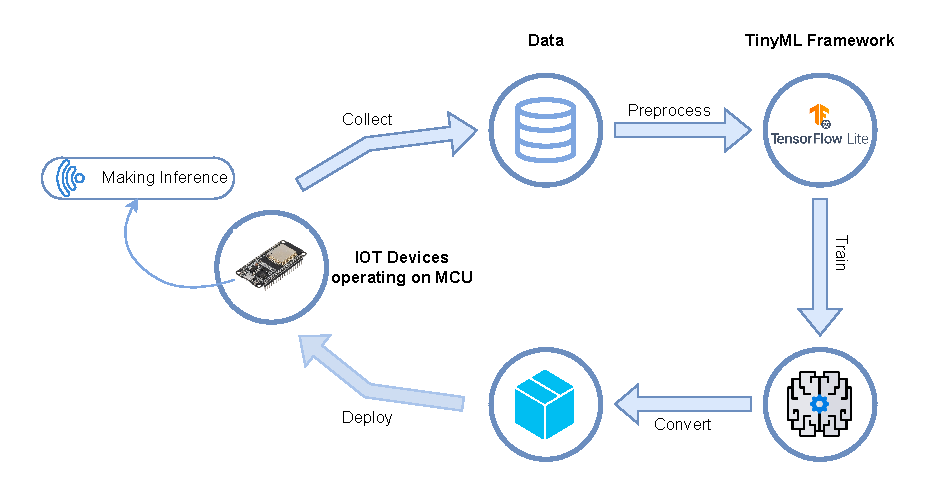
\includegraphics[width=1\columnwidth]{resource/tinyml_deployment.pdf}
	}
	\caption{TinyML Deployment pipeline}
	% A label to allow refering to this figure in the text.
	\label{TUM}
\end{figure}

\section{TinyML Overview} 
\label{tinyml_overview}

\subsection{Key Concepts and Techniques}

Pruning removes unnecessary neurons or connections from a neural network to reduce its size and complexity. This optimization lowers memory and computational demands, making the model faster and more efficient for deployment on resource-limited devices like microcontrollers.

Quantization reduces the precision of model parameters (e.g., from 32-bit to 8-bit), which decreases model size and computational needs. This technique enables efficient model inference on devices with limited memory and processing power, such as those used in TinyML applications.

With the TinyML model running on edge, the data is stored, processed and analysed internally rather
than at an external server or cloud. 

\subsection{TinyML pipeline}



\paragraph{Data Collection:}
	The workflow starts with collecting data from an IoT device. This data serves as the input for training machine learning models. The IoT device can gather various types of data depending on the application, such as sensor data in smart homes or environmental monitoring. \\[0.10cm]
\paragraph{Preprocessing:}
	After collecting data, it moves to the preprocessing stage. Here, the data is cleaned and prepared for model training. Preprocessing can involve tasks such as normalization, handling missing values, or feature extraction to improve the quality of the input data.\\[0.10cm]
\paragraph{Model Training:}
	The preprocessed data is fed into an ML framework, where a machine learning model is trained. This stage involves using machine learning algorithms to find patterns in the data, building a predictive or analytical model that can generalize from the data.\\[0.10cm]
\paragraph{Model Conversion:}
	Once the model is trained, it is converted into a format suitable for deployment on resource-constrained devices, like microcontrollers. This step might involve techniques such as quantization (reducing the precision of model weights) or pruning (removing unnecessary parts of the model) to reduce the model’s size and computation needs.\\[0.10cm]
\paragraph{Model Packaging:}
	After conversion, the model is packaged into a deployable form. This includes bundling the model with any necessary runtime components to allow it to be executed efficiently on the target device.\\[0.10cm]
\paragraph{Deployment:}
	The next step involves deploying the packaged model onto an IoT device. This means transferring the model to the device, setting it up for real-time inference or operation in the field.\\[0.10cm]
\paragraph{Inference:}
	Finally, the deployed model performs inference on the IoT device. Inference refers to the process of using the model to make predictions or decisions based on new data collected by the IoT device. The model operates locally on the device without needing continuous cloud connectivity, enabling real-time decision-making at the edge.\\[0.10cm]



\section{Enablements of TinyML in Industrial Setting}
\label{prod_tinyml}

\subsection{Challenges}

The fundamental pipeline for deploying a TinyML model to a microcontroller, as described above in Chapter~\ref{tinyml_overview}, provides a general framework for model development and deployment. However, in industrial settings, this pipeline often falls short due to a variety of challenges unique to production environments. Firstly, industrial applications typically demand more robust and adaptable systems, requiring continuous model updates and seamless integration within complex IoT infrastructures. Secondly, these demands introduce specific obstacles, such as the inability to regularly update models on resource-constrained devices and the difficulty of integrating TinyML systems with existing IoT architectures.

\subsubsection{Adaptation to unseen scenarios and constantly changing conditions}
In traditional machine learning (ML), models can be regularly updated with new data through a constant internet connection, allowing them to stay relevant as conditions evolve. This capability, however, is often unavailable for TinyML models deployed on microcontroller units (MCUs) in IoT or edge devices, which typically lack continuous internet access. Consequently, once a model is deployed on an MCU, it may remain static for extended periods, operating without the benefit of regular updates.

This static deployment significantly impacts TinyML models over time, especially in dynamic environments where data patterns evolve. In real-world applications, conditions rarely remain constant, and the input data the model receives can change due to factors such as seasonal variations, environmental shifts, or user behavior changes. Without regular updates, a static model can struggle to adapt to these evolving patterns, a challenge known as concept drift (when the relationship between input and output changes) and data drift (when the distribution of input data changes). Both forms of drift can lead to a decline in model performance, making it essential to consider ways to address these challenges in TinyML deployments.


\subsubsection{Integrating with Existing IOT System and Management of TinyML Models in Hetegenous Devices}
Integrating TinyML-enabled microcontrollers (MCUs) into existing IoT systems presents several unique challenges. IoT infrastructures are often built on established architectures, protocols, and data formats that may not be directly compatible with TinyML MCUs. Adapting these MCUs to work within the existing IoT ecosystem requires significant customization to ensure seamless data exchange, communication, and interoperability.

Moreover, existing IoT systems frequently rely on centralized processing or cloud-based analytics, while TinyML emphasizes local computation on edge devices. This architectural shift introduces complexities in synchronizing data and managing hybrid workflows that combine cloud and edge processing. Industrial IoT deployments also come with strict security and compliance requirements, so integrating TinyML MCUs necessitates additional security protocols, device authentication, and data encryption to maintain data integrity across the IoT network.

Maintenance and scalability issues can complicate the integration of TinyML into IoT systems at scale. Updating models on distributed MCUs, managing firmware compatibility, and monitoring device health require robust infrastructure and automated processes, adding layers of complexity to deploying and managing TinyML solutions within existing IoT frameworks. Moreover, to manage and operate such sophisitcated system requires deep technical capability which many of professionals with good domain lacks. This urges not only the need for effective methods to manage and maintain TinyML systems at scale but also the importance of making these systems accessible to a broader range of professionals.Enabling more individuals to work with TinyML systems will be crucial for ensuring widespread adoption and operational success in industrial environments. \cite{hussein_original_2024, paul_rethinking_2021, de_prado_robustifying_2020,ren_synergy_2021,roshan_adaptive_2021}.


\subsection{Bringing tinyML to production environment}

In order to target each of the outlined challenges, we have found in recent researches the following approaches proposed by Ren et al. \cite{ren_tinyol_2021, ren_how_2022, ren_device_2024}.

\subsubsection{Advanced On Device Learning Methods}
Creating a general NN model for general use is impractical for MCUs due to their resource-constraint nature. A simple NN model can easily exceed the hard storage room of a MCU. Moreover, for a general NN model to function, it needs to be updated with field data on the fly, which usually not possible as MCUs do not possess constant connection to the internets, especially while operating at edge.

In their paper on TinyOL (Tiny Machine Learning with Online Learning), Ren et al. introduced a novel system that enables on-device learning. This approach allows models deployed on embedded devices, such as sensors or microcontrollers, to learn and adapt in real time without requiring external retraining.

\begin{figure}
	\centerline{
	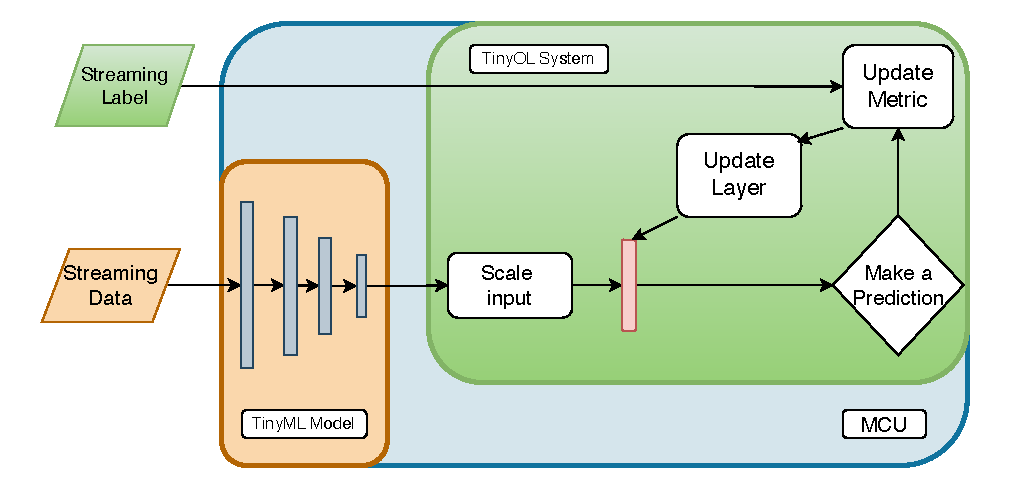
\includegraphics[width=1\columnwidth]{resource/tinyol_on_mcu.pdf}
	}
	\caption{TinyOL Components on MCUs (adapted from Ren et al.)}
	% A label to allow refering to this figure in the text.
	\label{TinyOL}
\end{figure}

The core of TinyOL lies in the additional layer marked in red in Figure~\ref{TinyOL} reffered to as the \textbf{update layer} which consists of neurons that can be customized, initialied, and updated on the fly. This layer serves as an output layer that can adapt to new data while preserving the original network's structure. Following is the breakdown of the other components in Figure~\ref{TinyOL}.

\begin{itemize}
    \item \textbf{Streaming Data}:
    This component represents the live data input collected by the MCU from its environment. It is fed into the TinyML model continuously, allowing the system to make predictions based on real-time information.

    \item \textbf{TinyML Model}:
    The core machine learning model deployed on the MCU. It takes streaming data as input and performs initial processing. This model consists of several layers (depicted by vertical bars), which extract features from the data.

    \item \textbf{Scale Input}:
    After the TinyML model processes the input data, it passes through a scaling component. This step standardizes or normalizes the data to ensure it fits the model’s expected input distribution, helping maintain consistent performance as new data arrives.

    \item \textbf{Make a Prediction}:
    After scaling and processing, the TinyOL system uses the model to make predictions. This decision node represents the point at which the system outputs a result based on the latest input data.

    \item \textbf{Update Metric}:
    When true labels (ground truth) are available, the system can update evaluation metrics based on the prediction’s accuracy. This component helps measure model performance and provides feedback for updating the model’s parameters.

    \item \textbf{Streaming Label}:
    This component represents the true labels or ground truth data available intermittently. When available, it is used to calculate metrics and adjust the update layer, enabling the model to correct itself over time and adapt to changing data patterns.
\end{itemize}


\paragraph{TinyOL Workflow}
The \textbf{TinyOL workflow} is summarized in the authors' algorithm \cite{ren_tinyol_2021}. The workflow proceeds as follows:
\begin{enumerate}
    \item \textit{Initialization:} TinyOL initializes both the TinyML model and the TinyOL system for on-device learning.
    \item \textit{Streaming Data Processing:} As new data points are received from the data stream, TinyOL processes each sample iteratively.
    \item \textit{Normalization and Standardization:} The running mean and variance of the incoming data are updated for standardization purposes, preparing the data for the model.
    \item \textit{Prediction and Model Update:} TinyOL uses the standardized input to make a prediction. If a true label is available, TinyOL computes the error between the prediction and the label, updating evaluation metrics. The model’s weights are then adjusted accordingly using techniques such as \textbf{stochastic gradient descent (SGD)}.
\end{enumerate}

\paragraph{Minium Resource Consumption:}
After processing each data point, TinyOL discards it to conserve memory. Compared to traditional batch/offline training methods, this efficient approach enables TinyOL to handle high volumes of streaming data, which is essential for resource-constrained MCUs with limited storage and processing capacity. The framework operates with as little as 7 KB of RAM and 135 KB of Flash memory.

\paragraph{Continuous Adaptation:}
TinyOL’s architecture allows it to continuously adapt to new data patterns over time, addressing issues like \textbf{concept drift} and \textbf{data drift}. By updating model weights in real time, the system ensures that the deployed model remains relevant and can handle changes in input data characteristics that may not have been present during initial training.

\subsubsection{Management of TinyML systems at scale}

There has been increased attention to TinyML Management with differents methods proposed such as: TinyML as a service , Model Card to describe and organize the information of trained models \cite{mitchell_model_2019}, or TinyML Operations (TinyMLOps) \cite{antonini_tiny-mlops_2022} to build an abstraction layer for various hardware compilers. However, theses approaches reveal certain drawbacks as they lack features for users to store and exchange information about existing resources. 

The paper introduces a TinyML low-code management framework called SeLoC-ML (Semantic Low-Code ML), designed to simplify the deployment, management, and scaling of TinyML applications. The essentials of SeLoC-ML can be broken down into two main parts: to build a KG ontology on the existing overal TinyML system and to inject the KG into a low-code platform \footnote{A low-code platform is a development environment that enables application creation through visual interfaces and minimal coding, making it accessible to users with limited programming knowledge. \url{https://www.ibm.com/topics/low-code/}}. 


\begin{figure*}[t]
	\centerline{
	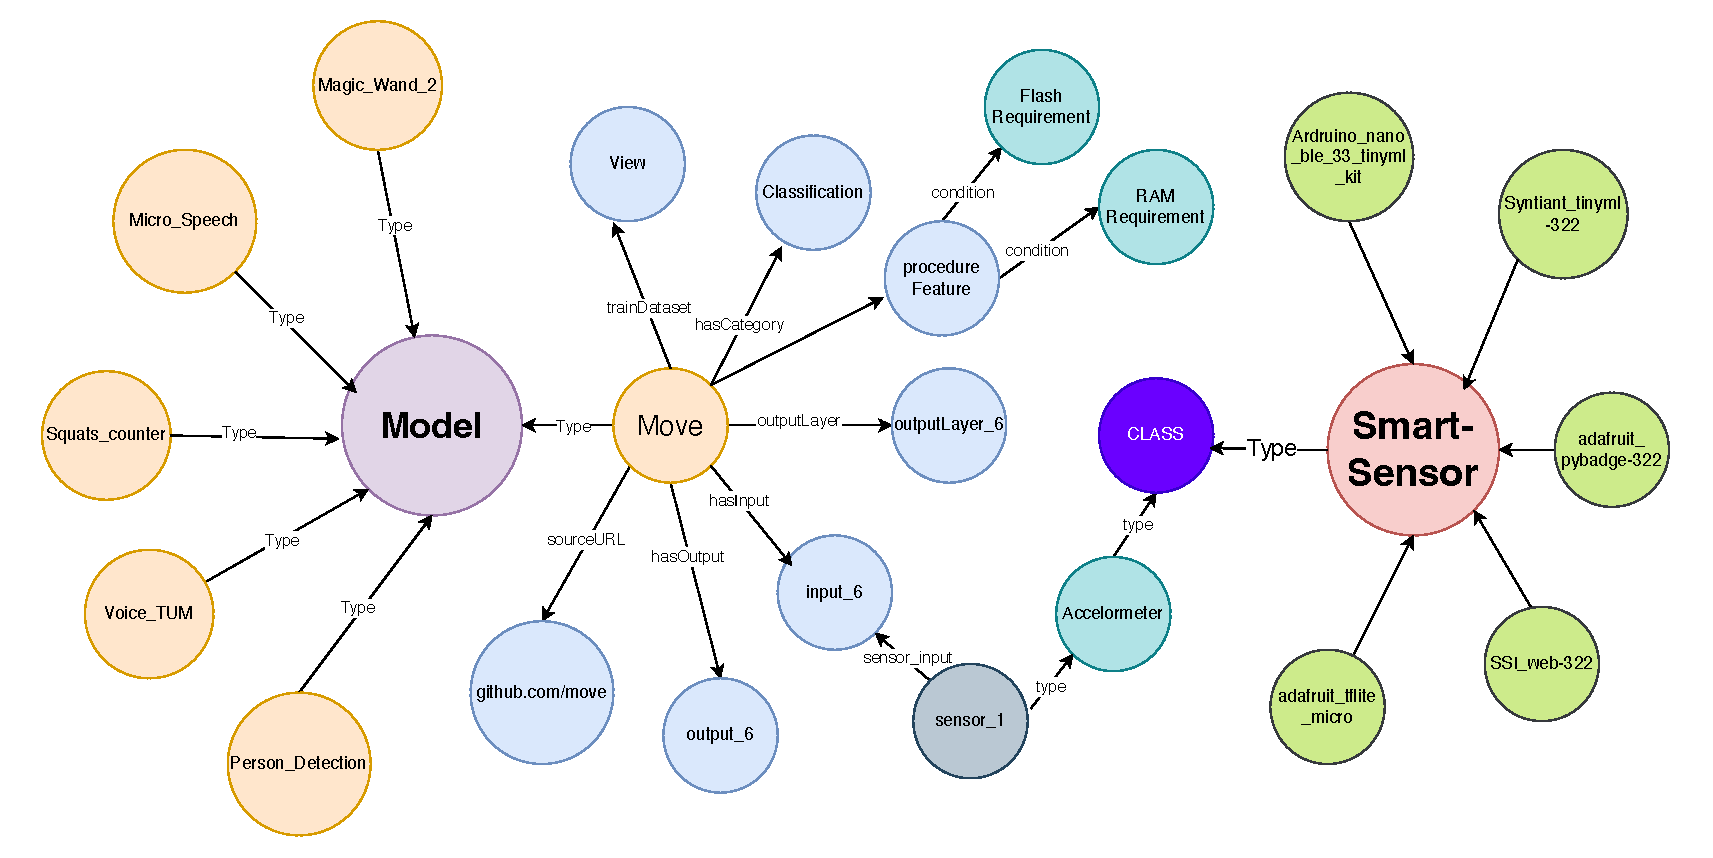
\includegraphics[width=0.9\textwidth]{resource/KG.pdf}
	}
	\caption{Visualization of System's Knowledge Graph (Simplified)}
	\label{KG}
\end{figure*}


\paragraph{Contruction of the Knowledge Graph (KG):} 

By reusing existing standards, like the \textbf{Semantic Sensor Network(SSN)} and \textbf{W3C Thing Description (TD)}  \footnote{\url{https://www.w3.org/WoT/}}
ontologies (a structured schema), an ontology that includes defitions and metadata for TinyML models, such as neural network architecture, layer configurations, and hardware requirements can be built. These data then can be stored using a graph database to facilitate management, dicovery, and deployment of TinyML applications.

Figure \ref{KG} is a simplified visual example of a knowledge graph. A total of 6 ML models are shown on the left side of the figure. One model is especially displayed in details. The "Move" model, as depicted in the knowledge graph, represents a TinyML motion-detection or activity-recognition model with defined input and output requirements, metrics, and compatibility conditions. By including this model in the knowledge graph, the TinyML management system can ensure the Move model is deployed on compatible hardware, facilitating real-time motion analysis or gesture detection in various applications. On the right-side cluster represents various IoT devices or sensor types, each represented by green nodes labeled with device names like “arduino\_nano\_ble\_33” and “adafruit\_tflite\_micro.” Finally, the link from Smart Sensor to Move Model in the knowledge graph represents a data dependency and compatibility relationship. It indicates that for the Move Model to function effectively, it requires input from a device that fits the description of a Smart Sensor.

\paragraph{Integrating into a low-code platform:}
Having the knowledge graph in form of a graphDB contructred, next step is to integrate with a low-code platform, to enable non-experts to manage and deploy TinyML models across diverse embedded devices. There are several different low-code plattforms in the market such as: SAP Build \footnote{\url{https://www.sap.com/products/technology-platform/build.html}} or Siemen Mendix \footnote{\url{https://www.mendix.com}}. Low-code software development cuts down on coding by using simple, drag-and-drop visual tools. This makes it quick to build, easy to update, and straightforward to manage business applications without needing much programming experience.



This approach addresses the challenges of \textbf{updating models on distributed MCUs} and \textbf{managing firmware compatibility} by leveraging Semantic Web technologies and a Knowledge Graph (KG) to centralize and standardize information about TinyML models and IoT devices. The framework’s \textit{ontology} provides a standardized way to describe ML models and IoT devices, facilitating tracking of model versions, configurations, and updates across various devices. By storing information about model updates, dependencies, and compatibility requirements in the KG, the system enables automated discovery of compatible models for each device, allowing administrators to push updates more efficiently. The \textit{querying capabilities} of the Knowledge Graph make it easy to identify which MCUs require updates, simplifying model deployment across large-scale, distributed systems. Additionally, the KG maintains details about each device’s firmware, hardware specifications, and compatibility requirements, ensuring that only compatible firmware and model updates are deployed. This centralized approach minimizes the risk of deploying incompatible firmware or models, which is crucial in environments with diverse MCU configurations. 


\section{Use Cases of TinyML in Industrial Setting}
\label{use_cases}

\subsection{Industrial Predictive Maintenance}

Predictive Maintenance (PdM) refers to a practice where business, based on series of historical and failure data, to predict in the future potential health and availability of aquiqments as well as anticipate defects in advance before they occur, thereby increase equipment lifespan, reduce downtime and operating cost \cite{ooko_application_2024}. The practice of consantly observing and predicting has its own inherent flaws and challenges such as financial and organizational constraints, limited source of historical data, and deployment of suitable PdM model \cite{zonta_predictive_2020}. 

TinyML offers a promising solution to several challenges by enabling intelligent predictive maintenance through embedded, low-power machine learning algorithms that can process data directly on the device. Unlike traditional ML in PdM, which typically relies on centralized data centers and cloud infrastructure, TinyML method helps close the gap in deploying predictive maintenance models by reduce the dependence on large-scale data infrastructure and addressing data source and computational limitations \cite{abadade_comprehensive_2023}. By allowing edge devices to process and analyze data locally, TinyML reduces the need for extensive data transmission and storage \cite{ooko_tinyml_2021}. This enhances the efficiency and reliability of IoT systems by ensuring that only relevant, actionable insights are sent back to the central system.

\subsubsection{TinyML vs. Standard ML}

According to \cite{achouch_predictive_2022,zonta_predictive_2020}, there are 80\% solutions for PdM found in literatures are ML-based and only 20\% are TinyML-based. This shows that the TinyML-based solutions in industry are still under-discovered as it still has certain weaknesses compared to Standard ML approaches.

Standard ML models operation requires a lot more computational power, however, as result, are able to hanlde complex sitations at higher accuracy. On the other hand, Standard ML performs with high latency and power consumption, due to the need to transmit data to servers which poses security breaches.

\subsubsection{Use Cases in PdM}

\paragraph{Anomaly Detection}
\paragraph{Operational Monitoring and Analysis}
\paragraph{Health and Condition Monitoring}
\paragraph{Predictive Maintenance}



\subsection{Smart Agriculture}
TinyML is poised to play a crucial role in the future of smart agriculture. By enabling real-time, on-device data processing and decision-making, TinyML is empowering farmers to optimize resource usage, increase productivity, and promote sustainable farming practices. As the technology continues to evolve, we can expect to see even more innovative applications of TinyML in agriculture, contributing to global food security and environmental sustainability.
\cite{tsoukas_tinyml-based_2023} presents a smart agriculture system based on tinyML and why tinyML can solve some of the long-existing challenges of agriculture.

\footnote{\url{https://github.com/SaiJeevanPuchakayala/FarmWiser}}
\subsubsection{Precision Agriculture}

\paragraph{Soil Monitoring}
\paragraph{Crop Health Monitoring}
\paragraph{Weather Monitoringg}
\footnote{\url{https://blues.com/use-cases/smart-farming-with-iot-and-machine-learning/}}

\subsubsection{Resource Optimization}
\paragraph{Smart Irrigation}
\paragraph{Precision Fertilization}

\subsubsection{Automated Farming Operations}



\subsection{Healthcare Monitoring}

\subsubsection{Wearable Health Monitoring Devices}
\paragraph{Chronic Disease Management:}TinyML-powered wearables can monitor vital signs such as heart rate, blood pressure, and glucose levels in real-time. This allows for continuous assessment of patients with chronic conditions like diabetes or hypertension, enabling timely interventions and personalized treatment plans.
\paragraph{Early Detection of Health Anomalies:}Devices equipped with TinyML can detect early signs of health issues by analyzing patterns in physiological data. For instance, changes in heart rate variability or oxygen saturation can be monitored to predict potential cardiac events or respiratory issues.
\paragraph{Fitness and Activity Tracking:}
Fitness trackers using TinyML can provide detailed analysis of physical activities, sleep patterns, and calorie expenditure. This data helps users maintain healthy lifestyles by offering personalized recommendations based on their activity levels.
Health care for factory workers - detection whether somebody about to faint

In conclusion, TinyML holds great promise for transforming healthcare monitoring by enabling real-time, personalized health insights through low-power wearable devices. As technology advances, its impact on improving patient care and outcomes is expected to grow significantly.


\section{Future of TinyML }
\label{future_of_tinyml}

The future of TinyML holds immense potential as it continues to evolve to meet the demands of diverse industrial applications. Key trends that are expected to drive TinyML's progress include advancements in model optimization techniques, integration with edge AI, and improvements in hardware capabilities. Enhanced techniques like federated learning for TinyML could allow devices to learn collaboratively without sharing raw data, addressing both data privacy and adaptability in dynamic environments. Additionally, further development in quantization, pruning, and neural architecture search will allow models to be more efficiently deployed on constrained devices, expanding TinyML’s applicability.

The expansion of 5G and the evolution of connectivity standards may also accelerate TinyML adoption, as these advancements could support more reliable intermittent connectivity for edge devices. This would facilitate more frequent model updates and allow TinyML models to synchronize with central systems when needed, even in remote areas. Another future direction is the integration of TinyML with the Internet of Things (IoT) on a larger scale, making real-time analytics accessible across widespread networks of low-power devices. TinyML is also expected to expand in areas like smart cities, environmental monitoring, and autonomous systems, where real-time data processing on edge devices is crucial. As the ecosystem grows, more low-code platforms and management frameworks, such as SeLoC-ML, will likely emerge, empowering a broader range of professionals to develop, deploy, and maintain TinyML systems effectively.

\section{Conclusion}
\label{conclusion}

TinyML represents a paradigm shift in deploying machine learning on resource-constrained devices, offering a feasible solution for real-time, low-power data processing directly on edge devices. This paper has highlighted the critical challenges and considerations in developing and deploying TinyML models in industrial settings, including the limitations posed by hardware, the need for continuous adaptation, and the complexities of integrating with existing IoT systems. Practical approaches such as on-device learning methods, like TinyOL, and management frameworks, such as SeLoC-ML, illustrate the ways in which TinyML can be efficiently scaled and managed to meet industrial demands.

The use cases discussed—spanning predictive maintenance, smart agriculture, and healthcare monitoring—demonstrate TinyML's transformative potential across industries, providing insights into its real-world applications and impact. While challenges remain, the ongoing advancements in hardware, model optimization techniques, and low-code platforms offer promising solutions to further simplify and enhance the deployment of TinyML systems. TinyML is well-positioned to continue expanding its impact, bringing intelligent edge computing capabilities closer to a wider range of industrial applications and enabling smarter, more efficient systems across the globe.



\bibliographystyle{plain}
% Literature sources are to be found in seminarpaper.bib
\bibliography{seminarpaper}
\end{document}
